\chapter{Physcis Objects}

\label{ch:objects}
This chapter introduced the physics objects used in this thesis in the reconstruction of events. 
 The reconstruction of primary vertices is described in Section~\ref{sec:pv}. 
The reconstruction of electrons, muons and taus are described in Section~\ref{sec:el}, Section~\ref{sec:mu} and Section~\ref{sec:taus}.
%Taus, which are also reconstructed as jets, are described in Section~\ref{sec:tau}. 
Different types of jets that are used by this analysis in different kinematic regions are described in Section~\ref{sec:jets}. 
The reconstruction of missing transverse energy (\met) and missing transverse energy significance, is discussed in Section~\ref{sec:met}. 
Finally Higgs tagging is described in detail in Section~\ref{sec:higgs}. 


\section{Inner Detector Tracks and Primary Vertex}
\label{sec:pv}
\par The tracks in the inner detector are based on fitting a trajectory model to a set of measurements using a sequence of algorithms
~\cite{Cornelissen:1020106}.
\par The inside-out algorithm, which is the baseline algorithm and is designed for efficient reconstruction of primary particles. 
It starts with three-point seeds in the silicon detectors and adds hits moving away from the interaction point using a combinatorial Kalman filter 
and tracks are extended into the TRT.
\par Then reconstruction of secondary particles produced by the interactions of the primary particles is achieved by Back-tracking. 
Back-tracking means a track search starts from segments reconstructed in the TRT and extends inwards by adding silicon hits. 
TRT-standalone tracks refer to tracks from TRT segment without extension into the silicon detectors.					
\par The transverse and longitudinal impact parameters of a track are referred to as $d_0$ and $z_0$ and their resolutions as $\sigma_{d_0}$ 
and $\sigma_{z_0}$. 
\par Each beam generates multiple track vertices, and the vertices are reconstructed from the available inner detector tracks.
\par All vertices with at least two associated tracks are retained as valid primary ver- tex candidates. 
The output of the vertex reconstruction algorithm is a set of three dimensional vertex positions and their covariance matrices. 
The primary vertex is selected as the one with the largest $\sum p_T^2$, where the sum is over all associated tracks. 
The basic track selection criteria are summarized in Table~\ref{tab:pv}.

\begin{table}[tbh]
\centering
\scriptsize
\begin{tabular}{|l|c|c}

\hline
 Aim& Selection \\
\hline
Reject soft fake tracks &$p_T> 0.4~GeV$ \\
\hline
In ID fiducial volume &$|\eta| < 2.5$ \\
\hline 
    Enough hits for track reconstruction & More than 9 hits between the Pixel\&SCT detectors for $|\eta|\le 1.65$\\
\hline 
    Enough hits for track reconstruction & More than 11 hits between the Pixel\&SCT detectors for $|\eta|\ge 1.65$\\
    
\hline 
 Good hit quality& Less than 2 hits in a SCT detector layer shared by multiple tracks\\
\hline 
 Good hit quality& Less than 1 hits in a Pixel detector layer shared by multiple tracks\\
\hline
 Good hit quality&0 missing hit in the Pixel detector when a hit is expected\\
\hline 
Good hit quality&Less than 1 missing hits in the SCT detector when hits are expected\\
 \hline
\end{tabular}
\caption{Selection criteria for track to reconstruct primary and pile-up vertices.}
\label{tab:pv}

\end{table}


\section{Electrons}
\label{sec:el}
\par Electron candidates are clusters of energy associated with ID tracks, 
where the final track-cluster matching is performed after the tracks have been fitted with a Gaussian-sum filter.
\par A few variables are checked to identify electron while suppressing background objects 
such as hadronic jets or converted photons~\cite{ATL-PHYS-PUB-2015-041}. 
They are the hits in the silicon detectors, including a hit on the IBL, and a likelihood discriminator, 
which combines the shower shape information provided by the highly segmented calorimeter, hits in the high-threshold TRT, 
compatibility of the tracking and calorimeter information, track quality information, 
as well as the impact parameter in the transverse plane ($|d_0|$) and its significance ($\frac{|d_0|}{\sigma_{d_0}}$).
\par Electron isolation measures the detector activity around an electron candidate, 
and can be used to further reject backgrounds such as electrons originating from converted photons produced in hadron decays, 
electrons from heavy flavor hadron decays, and light hadrons misidentified as electrons.
\par There are several working points of the likelihood variable which depends on how strict the requirements we require on electrons. 
This analysis uses the LooseLLHBLayer working point. In addition, this analysis applies two categories of electrons on electrons:
VHLoose and ZHSignal. The definitions of VHLoose and ZHSignal electrons are summarized in Table~\ref{tab:el}.
\begin{table}[tbh]
\centering
\begin{tabular}{|l|c|c|c|c|c|c|c}
\hline
Electron Type & $|p_T|$ & $|\eta|$ & $\frac{|d_0|}{\sigma_{d_0}}$ & $z_0\dot sin\theta$ & Likelihood & Isolation \\
\hline 
VHLoose &$>7$&$<2.47$&$<5$&$<0.5$&LooseLLHBLayer&LooseTrackOnly\\
\hline 
ZHSignal&$>7$&$<2.47$&$<5$&$<0.5$&LooseLLHBLayer&LooseTrackOnly\\
\hline

\end{tabular}
\caption{Definitions for the different categories of electron.}
\label{tab:el}
\end{table}
\par The VHLoose definition is used in the Signal Region where ZHSignal definition is used in some Control Regions, since the VHLoose definition is looser.
 
\section{Muons}
\label{sec:mu}
\par Muon reconstruction is performed based on information from the inner detector (ID), Muon S and calorimeters. As instructed in~\cite{Aad:2016jkr}, 
there are five types depending on different reconstruction methods.

\begin{itemize}
\item Combined muons are reconstructed by combining the hits of the ID track and MS track and the energy loss in the calorimeter;
\item Segment-tagged muons are formed from a track in the ID if it is associated with at least one track segment in the MDT or CSC chambers. 
 It capture muons passing only one layer of MS chambers, due to their low \pt~or reduced MS acceptance in the region.
\item Extrapolated muons are reconstructed based only on the MS track and a loose requirement on compatibility with originating from the IP. 
 They are used to extend the acceptance for muon reconstruction into the region $2.5 <\eta< 2.7$. 
 The muon is required to traverse at least two layers of MS chambers to provide a track measurement, but three layers are required in the forward region.

\item Calorimeter-tagged muons. In the region of $|\eta< 0.1$, ID tracks with $15 ~GeV < p_T < 100 ~GeV$ are identified as muons if their energy deposits in the calorimeter 
 match with minimum ionizing particles. They recover muon acceptance in the region where the MS is only partially instrumented.

\end{itemize}
\par Similar to Electron reconstruction, there are different muon identification working point. This analysis chose ``Loose'', defined as muons reconstructed using any reconstruction methods, 
and ``Medium'', reconstructed using either the Combined muon or Extrapolated muon methods.
\par The VHLoose definition is used in the Signal Region where ZHSignal definition is used in some Control Regions, since the VHLoose definition is looser.					
\par As showed in Table~\ref{tab:mu}, this analysis applied additional criteria to muons in different regions. 
A tighter selection is required in Control Regions for a high muon purity and a looser selection when muons are not desired and are vetoed in the Signal Region.
\begin{table}[tbh]
\centering
\begin{tabular}{|l|c|c|c|c|c|c|c}

\hline
  Electron Type & $|p_T|$ &$|\eta|$ & $\frac{|d_0|}{\sigma_{d_0}}$&$z_0 sin\theta$ & Likelihood &Isolation \\
\hline 
VHLoose &$>7$&$<2.7$&$<3$&$<0.5$&Loose&LooseTrackOnly\\
\hline 
WHSignal &$>25$&$<2.5$&$<3$&$<0.5$&Medium&FixedTrackTTTight\\
\hline 
ZHSignal &$>25$&$<2.5$&$<3$&$<0.5$&Loose&LooseTrackOnly\\
\hline
\end{tabular}
\caption{Definitions for the different categories of muons.}
 \label{tab:mu}
\end{table}


\section{Taus}
\label{sec:taus}
% Tau, what and why
\par Tau lepton veto algorithm is needed in the analysis since it is not interested in the signal events. Tau particle, unlike its lighter lepton buddy, electron and muon, 
is the only lepton that can decay into hadrons. The branching ratio of hadronically tau decay is approximately 64.79\%. Therefore, it is important to reject hadronically decayed 
tau events in the hadronic analysis.

% How to reject tau with Loose Tau ID
\par Hadronicallly decayed tau can be reconstructed as small-radius jets and identified with a tree-based machine learning algorithm. A typically hadronically decayed tau jet 
can be characterized with either one or three charged hadrons, which can be applied to the tree-based classifiers to differentiate from QCD jets. With the trade-off of selection 
efficiencies and fake rate, three classifiers, loose, medium, tight, can be determined. More details can be found in \cite{ATL-PHYS-PUB-2015-045}. 
In order to reduce the hadronically decayed tau to a maximum extent, the loose working point is chosen to build the tau veto condition, together with the baseline section of $p_T > 25 GeV$ and $|\eta| < 2.5$.

\section{Jets}
\label{sec:jets}
\par In pp collisions, almost immediately after being produced, a quark or gluon fragments and hadronises, leading to a collimated spray of energetic hadrons -- 
a jet~\cite{Salam:2009jx}. There exist many different jet clustering algorithms to measure the jet properties. 
\par Among all jet finding algorithms, the anti-$k_T$ algorithm~\cite{Cacciari:2008gp} is most commonly used. This algorithm flavors clusterings that involve hard particles, 
and the jets then grow outwards around hard ``seeds''. R is in the denominator of the clustering distance metric. It determines the radial size of the jet in $\eta-\phi$ plane.
\par Calorimeter jets are reconstructed by combining topological clusters of energy deposits in the calorimeter~\cite{Aad:2011he}, while the inputs to track jet clustering are inner detector (ID) tracks. 
The small R = 0.4 calorimeter jets are used for b-quark reconstruction in the resolved topology. For jets that are from collimated decay products of heavy particles or low \pt~gluons, 
a large cone size are used to contain all of the decay products. Large-R jets are defined in ATLAS collaboration as jets reconstructed with the anti-$k_T$ algorithm with R = 1.0 using calibrated 
calorimeter clusters.The large R calorimeter jets are used for Higgs boson reconstruction in the boosted topology in this analysis.
\par In this iteration of the analysis, the variable radius track jet replaced the small fixed R = 0.2 track jets to be used for b-quark identification inside the large-R jets.

\subsection{Calorimeter jets}
\label{sec:calo}
 \par Topological clusters (topo-cluster) are cells are clustered together to reconstruct such particle shower, due to fine granularity in calorimeters. 
 The topo-cluster reconstruction is based on cell signal significance S/N, defined as the ratio of cell energy at electromagnetic energy scale over average expected noise. 
 The reconstruction starts from a seed cell with signal significance above the threshold of S/N = 4. Then the neighbouring cells with signal significance over S/N = 2 are included iteratively.
 Finally, all calorimeter cells neighbouring the formed topo-cluster are added. After the iteration, one outer layer of all surrounding cells are added, 
 so the resulting topological cluster is at the electromagnetic scale.
\par For large R jets, a local hadronic calibration (LCW) is then applied at cluster-by-cluster level to correct for non-compensation effect which underestimating the energy of hadronic particles.
For small R jets, EM scale becomes the default for ATLAS in Run 2.
\begin{figure}[htbp]
    \centering
    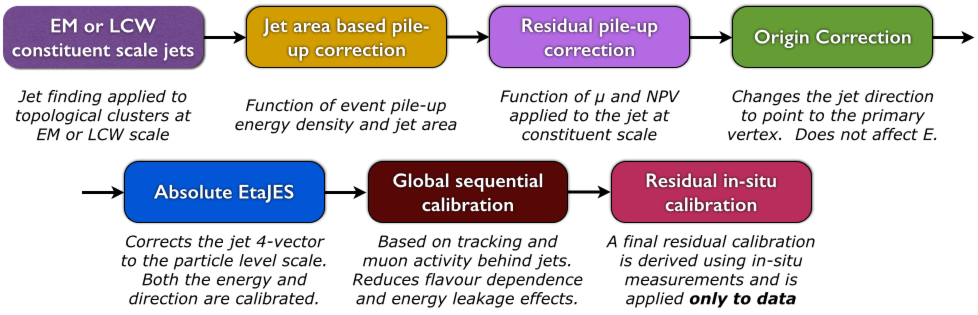
\includegraphics[width=1\textwidth]{chapters/c5/figures/jet_calib}
    \caption{Calibration stages for reconstructed jets.}
    \label{fig:jet-calib}
\end{figure}
\par After jets are reconstructed, calibration needs to be applied on the four momentum of reconstructed jet to restore it back to particle-level energy scale.
A series of calibrations are applied after jet clustering as shown in Fig~\ref{fig:jet-calib}.

\begin{itemize}
\item \textbf{Origin correction} The kinematic observables of each topo-cluster are recalculated using the vector from the primary hard-scattering vertex to the topo-cluster centroid as its direction. The resolution of $\eta$ can be improved in this step. The jet energy is unaffected.
\item \textbf{Jet area-based pile-up correction} This step are designed to remove the excess energy from pile-ups. The area-based \pt~density subtraction is applied event-by-event~\cite{Cacciari:2007fd}. The \pt~density is estimated using the medium of \pt~density of all jets in the event calculated by \pt/A, where A is the jet area.
\item \textbf{Residual pile-up correction} A residual \pt~dependency on in-time pile-up $N_{PV}$ and out-of-time pile-up $\mu$ is roughly linear. So the linear correction is applied with coefficients derived from MC simulation. 
\item \textbf{Absolute MC-based calibration} An absolute jet energy and $\eta$ correction is derived from MC simulation. The average energy response is defined as the mean of $E_{reco}/E_{truth}$ binned in $E_{truth}$ and $\eta_{jet}$. Similar correction is done for $\eta$. 
\item \textbf{Global sequential calibration} The global sequential calibration (GSC) method~\cite{Aad:2011he} is applied to improve resolution of JES. In this step, JES depends on five features which accounts for different aspects and the calibration factor is derived from MC. The procedure is similar to the absolute JES.
\item \textbf{Residual in situ calibration} This steps aims at correcting difference between data and MC. For jets up to 950 GeV and with $|\eta| < 0.8$, Z+jest and $\eta$+jet balance is used, while, for high-\pt~jet up to 2 TeV, multijet balance is used.
\end{itemize}
\par The larger the jet size, the more chances there are particles from underlying events, 
pile-up interactions and soft component of the radiation to contaminate the jet. Thus for large R jets, three techniques of jet grooming are developed:
split-filtering~\cite{Butterworth:2008iy}, pruning~\cite{Ellis:2009me} and trimming~\cite{Krohn:2009th}. 

\begin{itemize}
\item \textbf{Split-filtering} Large-R jets are first built with C/A algorithm. This algorithm includes splitting and filtering. 
 Splitting is to find the hard two-prong splitting substructure from massive parent particle. C/A jets are de-clustered by splitting jet into two pieces. De-clustering continues with the highest mass piece 
 until the requirements on mass-drop $\mu_{12} < \mu_{max}$ and momentum balance $\sqrt{y_{12}} > \sqrt{y_{min}}$ are met. 
 The momentum balance $y_{12} = \frac{min(p_{T1},p_{T2})}{m_{12}}\Delta R_{12} $ and mass-drop is defined as $\mu_{12} = max(m_1,m_2) m_{12}$, where $m_{12}$ 
 is the invariant mass of two pieces. If the requirements are not satisfied, the jet is discarded. Filtering aims at removing soft radiations that is irrelevant to the hard splitting process. 
 In filtering stage, constituents of surviving jet are reclsutered with subjet size of $R_{sub} = min(0.3,\Delta R_{12})$, where $\Delta R_{12}$ is taken from splitting stage.
\item \textbf{Pruning} Pruning is similar to trimming as it removes constituents with relative small $p_T$, while it has an additional wide-angle radiation veto. Large-R jets are first built with C/A or anti-$k_t$
 algorithm. Constituents of ungroomed large-R jet are then re-clustered with C/A algorithm based on $R_{cut}$ and $Z_{cut}$. In each pairwise clustering step, secondary constituents with wide-angle 
 $\Delta R_{12} > R_{cut} \times \frac{2M}{p_T}$ or soft property are discarded. Definition of being soft is that $f_2 < Z_{cut}$ where $f_2$ is the fraction of softer constituent \pt~with respect to the pair.
\item \textbf{Trimming} Large-R jets are first built with C/A or anti-$k_t$ algorithm. This requires reclustering all of the jet’s constituents using the $k_T$ algorithm, 
 which flavors clustering low \pt~constituents first. This creates a set of subjets with radius parameter $R_{sub}$. 
 Subjets with an energy below some threshold fraction of the energy of the large-R jet are removed from the large R jet. 
 The trimmed large-R jet will be used to reconstruct Higgs candidates in boosted region.
\end{itemize}
\par The resulting jet is trimmed large-R jets, and is used to reconstruct Higgs candidates when the b-quark decay products of the Higgs are too collimated to resolve by two small-R jets.

\par Small-R jets used in the analysis could be divided into two categories: central jets and forward Jets. Forward jets are small-R jets with $2.5 < |\eta| < 4.5$ and $p_T > 30 GeV$, and can be used by event selections to reduce backgrounds.
 Small-R jets with $|\eta| < 2.5$ and \pt~$> 20 GeV$ are called central jets and they are used to reconstruct Higgs candidates with low \pt~.
For central jets with $|\eta| < 2.4$ and $20 GeV < p_T < 60 GeV$, an additional requirement on jet vertex tagger value $JVT > 0.59$ are required. Details on the jet vertex tagger (JVT) is could be found here~\cite{Aad:2015ina}.



\subsection{Track jets}
\label{sec:track}


\par Track jets are jets built entirely from tracks reconstructed in inner detector via the same anti-$k_T$ algorithm as calorimeter jets. In Run 2, track jet b-tagging became the standard approach to resolve heavy flavor components from boosted decay of heavy resonances~\cite{ATL-PHYS-PUB-2015-035,ATLAS-CONF-2016-039}. Studies of track jet calibration can be found in~\cite{VanDenWollenberg:1981533}. 
\par In this thesis, two types of track jets are discussed. R = 0.2 track jets will be referred to as FR track jets, for fixed radius track jets, in contrast to the variable radius (VR) track jets which will be discussed later.

\par A track selection of input ID tracks is applied in order to suppress fake tracks and tracks from pile-up vertex. The selection criteria is summarized in Table~\ref{tab:trk}. With a relatively looser requirement on hits in the ID detectors compared to the track selection criteria for primary vertex reconstruction, it requires a small longitudinal impact parameter of the tracks with respect to the primary vertex to reject pile-up vertex.
\begin{table}	
\centering

    \scriptsize
\begin{tabular}{|l|c|c}
\hline
Aim & Selection \\					
\hline
Reject soft fake tracks &$p_T> 0.4 GeV$ \\
\hline
In ID fiducial volume &$|\eta| < 2.5$\\
\hline 
enough hits for track reconstruction & More than 7 hits between the Pixel and SCT detectors \\
\hline 
 good hit quality& Less than 1 hit in a Pixel shared by multiple tracks\\
\hline
 good hit quality&Less than 1 missing hit in the Pixel detector when a hit is expected\\
\hline 
good hit quality&Less than 2 missing hits in the SCT detector when hits are expected\\
 \hline
reject tracks from pile-up & $z_0 \dot sin(\theta) < 3 mm$\\
 \hline
\end{tabular}
\caption{Selection criteria for tracks to cluster track jets. }
\label{tab:trk}
\end{table}	
\par FR track jets are then built by applying anti-$k_T$ algorithm with R = {0.4, 0.3, 0.2} on selected tracks. Track jets in fiducial region with $p_T > 7 GeV$ and $|\eta| < 2.5$ are accepted as track jets with $p_T < 7 GeV$ are rejected as they are dominated by light jets~\cite{ATL-PHYS-PUB-2014-013}. 				
\par VR track jets are clustered using the anti-$k_t$ algorithm from tracks with the same selection criteria used for R = 0.2 track jets. The main feature of the VR track jet reconstruction~\cite{Krohn:2009zg}, compared to the FR jets is the \pt~dependence of the jet radius:
\begin{equation}
R \rightarrow R_{eff}(p_T) \approx \frac{\rho}{p_T}
\end{equation}
where the parameter $\rho$ shows how the effective jet radius scales with the \pt~of the pseudo-jet during the jet finding procedure, $R_{min}$ and $R_{max}$ are a lower and an upper cut on the jet radius.
To optimize the efficiency of double b-tagging over a wide mass, $ \rho = 30 GeV$, $R_{min} = 0.02$ and $R_{max} = 0.4$~\cite{ATL-PHYS-PUB-2017-010}.

\subsection{Ghost Association}
\label{sec:ga}

\par In practice, track jets are seldom used alone for object reconstruction and instead used along with the large calorimeter jets. Calorimeter jets are in charge of providing jet reconstruction while track jets are in charge of providing flavor tagging information. To match track jets to calorimeter jets is the first step for flavor tagging. 
\par Ghost association~\cite{Cacciari:2007fd,Cacciari:2008gn} is a method to associate the ``ghost'' (particles, jets or tracks) to jets by giving them negligible momentum and clustering them within the jets. This is to make sure that the hard-particle content of the jet is unaltered by the addition of the soft ghost particles during jet reclustering. The jet substructure after reclustering is unchanged compared to the previous jet, but with the addition of ``ghost'' as constituents.
\par An object (track, jet, truth particle) is ghost-associated to a jet if its ``ghost'' is clustered as a constituent of the jet.
\par Compared to $\Delta R$ association which matches objects based on angular distance, ghost association is more robust when dealing with overlapping jets or jets that are not cone-shaped.



\subsection{Flavor tagging}
\label{sec:track}
\par The identification of b jets is referred to as b-tagging or flavor tagging. After the fragmentation of b-quarks, about 70\% of the b-quark energy goes into the weakly decaying b-hadrons (~5 GeV). With an intrinsic life-time of $1.5 \times 10^{−12}$ s, the average decay lengths for b-hadrons of 30 GeV is about 3 mm, which could be measued with the high-precision tracking system in ATLAS.
The c-hadrons from b-hadrons decay also have similar average lifetimes, and thus leads to an additional decay. 
Several b-tagging algorithms are developed by studying the decay patterns. 				
\par ID tracks are used for these b-tagging algorithms, and tracks need to pass the basic quality cuts. 		
\par These three b-tagging algorithms below are used to provide complementary information and combined using boosted decision tree (BDT) to provide a score to distinguish between different flavors (c, b, light). 	
\begin{itemize}				
\item \textbf{Impact Parameter Based Algorithm (IP2D and IP3D)} 	
As shown in Fig.2 from the reference~\cite{ATL-PHYS-PUB-2015-022}, tracks from a displaced vertex have larger impact parameter than those coming from primary vertex. The probability density functions (PDFs) for the signed impact parameter significance of these tracks $\frac{d_0}{\sigma_{d_0}}$ and $\frac{z_0}{\sigma_{z_0}}$ are used to define ratios of the jet hypotheses of different flavors, and these are then combined in a single log likelihood ratio discriminant (LLR). While IP2D only uses transverse impact parameter, IP3D uses the 2D template with correlation between transverse and longitudinal direction.				
\par Both IP2D and IP3D assume that all tracks are independent and they are naive Bayesian models which ignore correlations between tracks. Besides, while it is easy to build 2D or 3D template histograms, it is technically hard to encode too many variables at the same time. To improve the results, new algorithm which makes use of the recurrent neural network with the same input tracks as IP2D/IP3D are developed in ATLAS b-tagging~\cite{ATL-PHYS-PUB-2017-003}. 
\item \textbf{Inclusive secondary vertex reconstruction algorithm (SV)} 	
The secondary vertex based algorithm explicitly reconstructs an inclusive displaced secondary vertex within the jet. Tracks passing quality cuts are first paired to form two-track vertex. And these two-track vertex would then be filtered to reject if coming from decay of long-lived particles such as $K_s$, $\Lambda$, photon conversion or hadronic interaction with detector materials. An inclusive secondary vertex would be fit using survived tracks using Kalman filter in an iterative way and certain quality cuts will be applied. 				
\item \textbf{Decay chain multi-vertex reconstruction algorithm (JetFitter)} 		 	 	 		The decay chain multi-vertex reconstruction algorithm is called JetFitter and studys the cascade decay structure of b-hadron and c-hadron coming out of it to reconstruct the hadron decay chain $Primary\ Vertex \rightarrow b \rightarrow c$ using a Kalman filter.		 	 	 		
\par Because unlike the SV algorithm, the vertex in JetFitter refers to the intersection between tracks and estimated decay chain direction and thus a vertex could have even only one track associated to it. Thus JetFitter typically has a much higher reconstruction efficiency, as well as a higher fake rate. To reduce the fake rate, a set of topological variables are built in JetFitter for discrimination purpose. 
\end{itemize}		

\par After running each b-tagging algorithms independently, output discriminative variables of each algorithm, as well as the kinematic properties of jets \pt~and $\eta$ are combined using BDT. The \pt~and $\eta$ joint distribution between signal and backgrounds re-weighted to match each other before training so that these kinematic variables are not treated as discriminative variables.
\par The training is performed on high purity ttbar and zprime MC samples with at least millions of events. While b-jets are used as signal jets, 
the background is a mixture of c-jets and light-jets. Three versions of mixture are available at ATLAS: MV2c00, MV2c10 and MV2c20. The number after character ``MV2c''
shows the percentage of c-jets in background mixture. 
Depending on the physics processes, users can choose the any of these three version.
The higher the number, the better the discrimination power against c-jets at the cost of less light-jet rejection. 
The performance of MV2c10 tagger~\cite{Varni:2655785} for discrimination against light-jet and c-jets can be found in Fig~\ref{fig:mv2c10}.

\begin{figure}[htbp]
    \centering 
    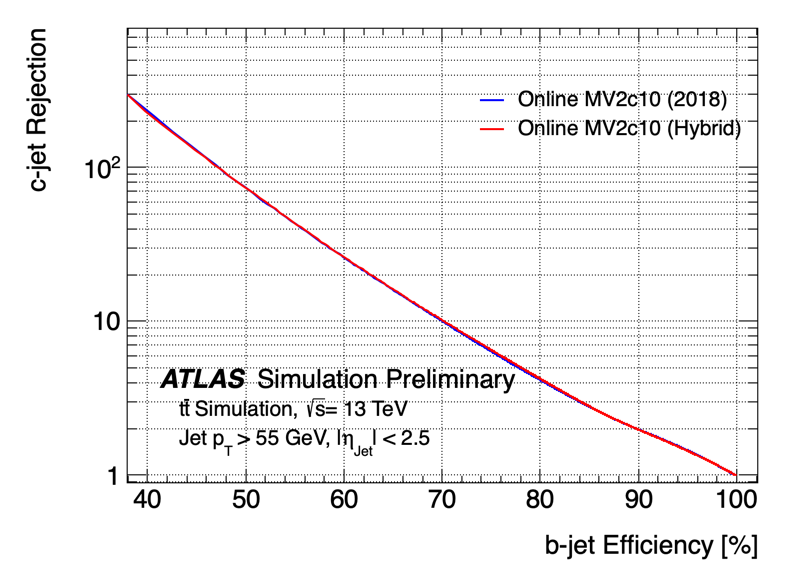
\includegraphics[width=0.4\textwidth]{chapters/c5/figures/ROC_cb}
    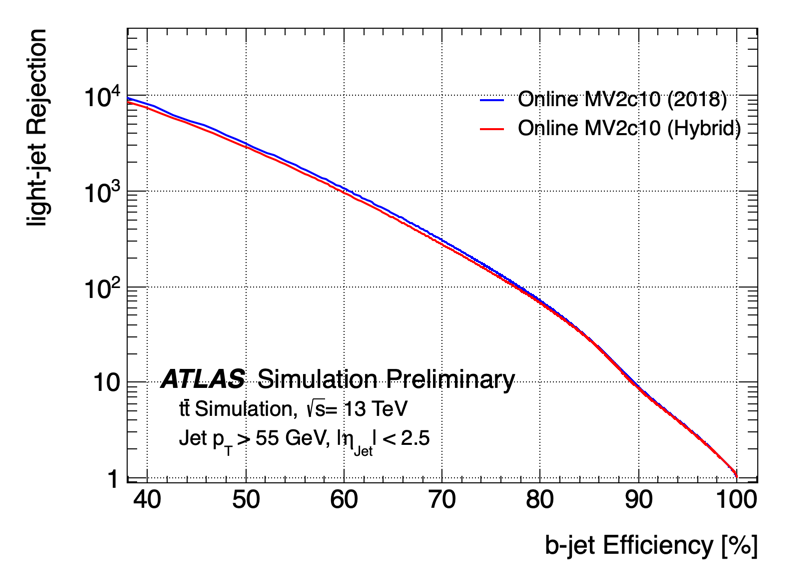
\includegraphics[width=0.4\textwidth]{chapters/c5/figures/ROC_lb}
    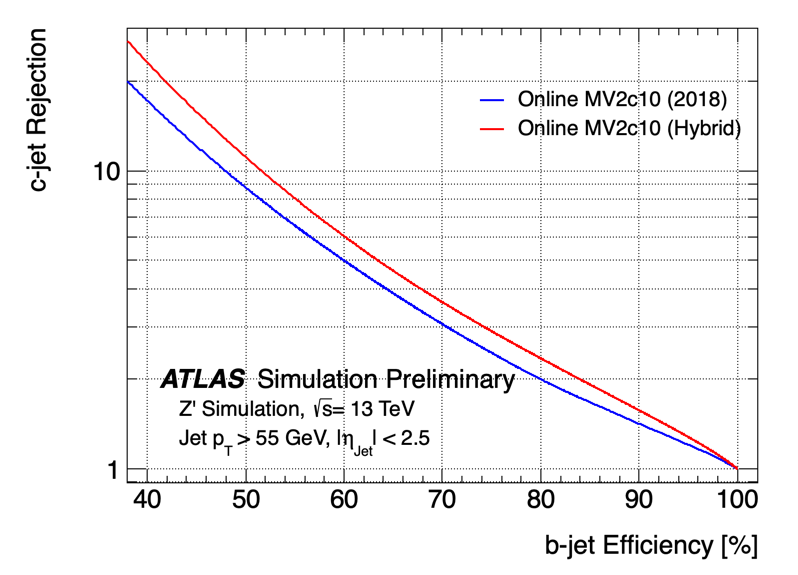
\includegraphics[width=0.4\textwidth]{chapters/c5/figures/ROC_cb_Zprime}
    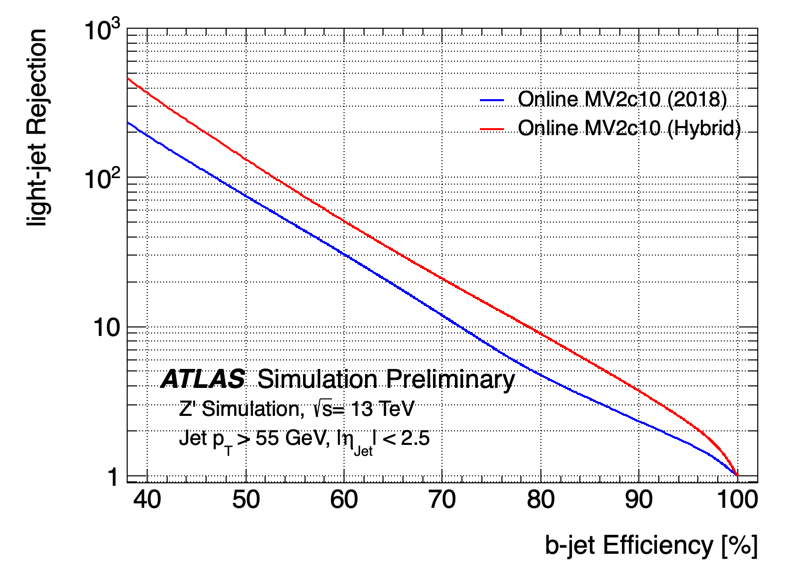
\includegraphics[width=0.4\textwidth]{chapters/c5/figures/ROC_lb_Zprime}
    \caption{Expected performance of \textit{b}-tagging algorithm (MV2c10) for \textit{b}-jet triggers in 2018 data-taking (blue solid line) is compared to the same \textit{b}-tagging algorithm trained on the Hybrid training sample (red solid line).}
    \label{fig:mv2c10}
\end{figure}

\section{Messing Transverse Energy/Momentum (MET) and Missing Transverse Energy Sigificance}

\label{sec:met}
% What is MET
\par According to the conservation of momentum, the sum of the transverse memento of all particles produced in collisions is zero. Considering the existence of the non-detectable object, the transverse energies from detected objects are not balanced. The unbalanced part of transverse momentum is called ''missing transverse energy''(\met), or MET for short.

% How to calculate MET with/without Tracker fully involved.
\par As mentioned in the last paragraph, the \met~is derived by all other detectable objects. The \met~calculation is the most difficult object not only because it needs a full calculation of all detectable objects from various detectors, but also from the small fraction of energy deposits from unclustered parts of detectors. As a result, the \met~scale and \met~resolution are affected by many factors, such as missing Muons, mismeasured Jets, beam pile-up, etc. In the ATLAS experiment, the \met~reconstruction uses energy deposits in the calorimeters and muons tracks reconstructed in the muon detectors. Trackers' information is also used to recover the low Pt fraction that missed in the calorimeters \cite{ATLAS-CONF-2013-082}. Therefore, both hard objects (high \pt~), like electrons, jets, muons, etc, and soft objects, like track soft terms, are considered in the \met~reconstruction.

% MET significance
\par The uncertainty of \met~calculation result can be remarkably large due to the complexity of the reconstruction algorithm. Therefore, a significance variable can be introduced to describe the reliability of the derived \met. The \met~significance is defined as
$$ S=\frac{\met}{\sqrt{\sum_{i}E_{Ti}}}, $$
where the numerator is the amplitude of derived \met, and the denominator is the scalar sum of the detected objects that used when to reconstruct the \met. A high value of \met~significance suggests the event is more likely to container invisible object rather than resolution smearing.

\section{Higgs tagging}
\label{sec:higgs}
\par For Higgs particle with sufficiently low \pt, two outcoming b-quarks can be reconstructed individually as Small-R = 0.4 calorimeter jets. However, for Higgs particle with high \pt, 
the two outcoming b-quarks are too collimated be reconstructed using small-R jets.
``Higgs tagging'' in the thesis refers to the techniques used to identify boosted Higgs decays to b-quarks. The Higgs candidate is reconstructed as a trimmed large-R jet 
with two ghost-associated b-tagged subjets, reconstructing the b-hadrons.
\subsection{Higgs tagging with advanced subjets}

\par Three techniques, variable radius track jet Higgs tagging technique, Exclusive-kT (ExKt) and Center-of- Mass (CoM), for tagging a very boosted Higgs 
particle~\cite{ATL-PHYS-PUB-2017-010}, 
whose b-hadron decay products will become too collimated to resolve even with R = 0.2 track jets.
\par The definition of VR track jets could be found in Section~\ref{sec:jets}, as showed in~\ref{fig:vr}. And the parameters $\rho = 30 GeV$, $R_{min} = 0.02$ and $R_{max} = 0.4$ 
are chosen after scanning different $\rho$ and radius as showd in Fig.~\ref{fig:vr-scan}.


ExKt subjet refers to exclusive regions of interest using exclusive-kT declustering of large-R jet. 
And CoM jets are constructed via exclusive-kT declusting in center of mass frame instead of in the lab frame.
\begin{figure}[htbp]
    \centering
    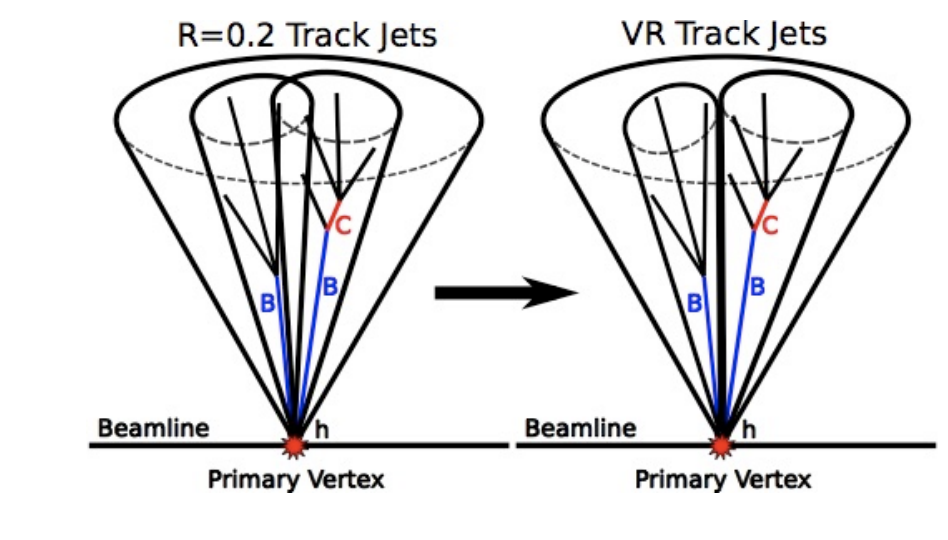
\includegraphics[width=0.6\textwidth]{chapters/c5/figures/VR}
    \caption{A cartoon depicting how using VR track jets instead of R = 0.2 track jets.}
    \label{fig:vr}
\end{figure}

\begin{figure}[htbp]
    \centering
    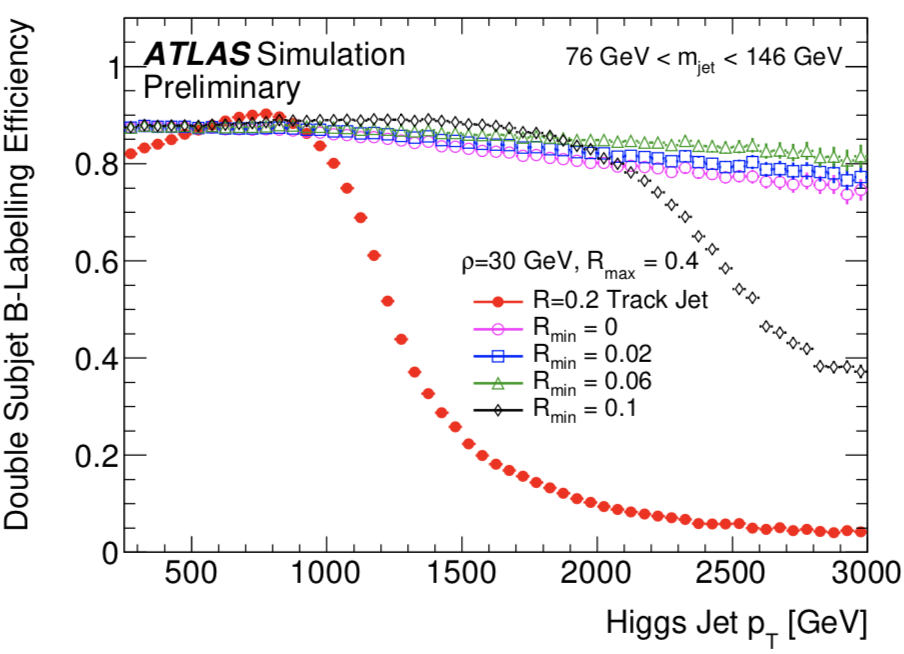
\includegraphics[width=0.4\textwidth]{chapters/c5/figures/r-vr}
    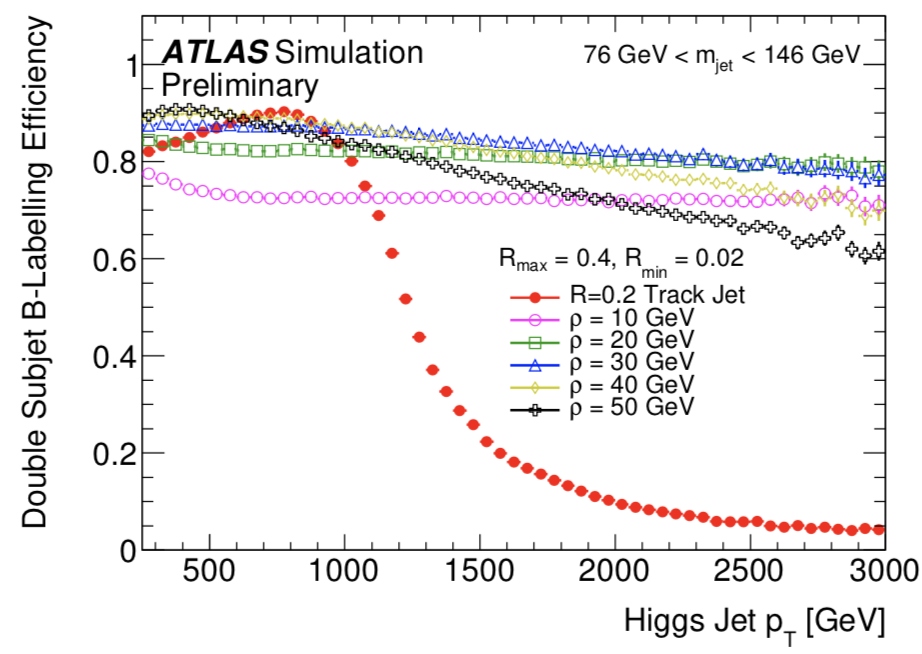
\includegraphics[width=0.4\textwidth]{chapters/c5/figures/rho-vr}
    \caption{Higgs effiency using two VR track jets with different R parameter (Left) and $\rho$ parameter (Right)} 
    \label{fig:vr-scan}
\end{figure}

\par The double subjets b-labelling performance for the FR track jet, VR track jet, ExKt and CoM techniques could be found in Fig.~\ref{fig:higgs_pt}.
The plot shows a dramatic decrease for the R = 0.2 track jet technique as the Higgs jet \pt~becomes larger than 1.2 TeV where this is precisely the region where the 
R = 0.2 track jets are expected to merge. 
New techniques, however, could reconstruct Higgs jets with a \pt~of 3 TeV. And receiver operating characteristic (ROC) curves showing the Higgs jet tagging performance versus 
QCD jet rejection are shown 
in Fig.~\ref{fig:higgs_ROC}.

\begin{figure}[htbp]
    \centering
    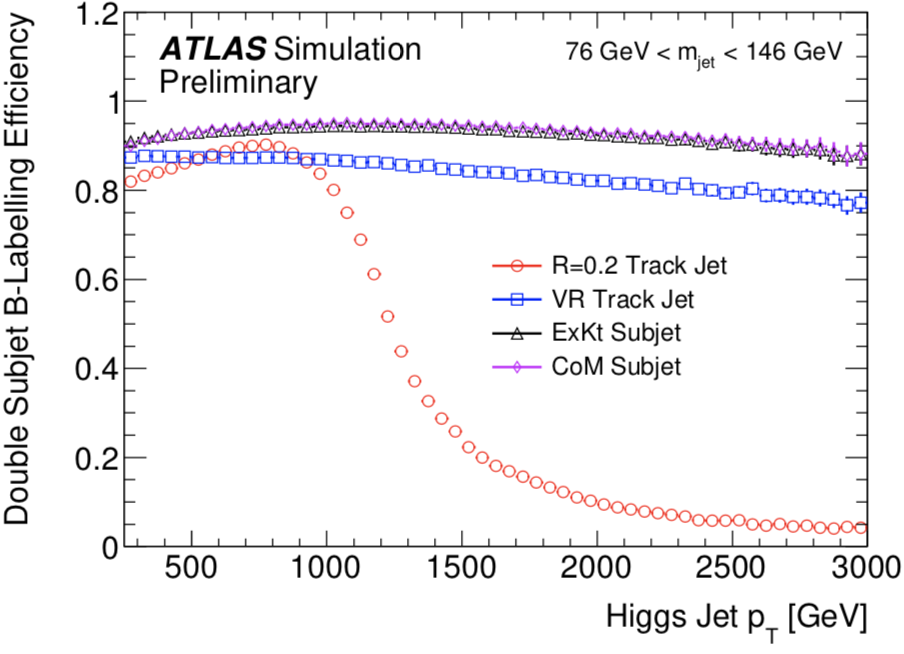
\includegraphics[width=0.6\textwidth]{chapters/c5/figures/higgs_pt}
    \caption{Higgs efficiency using four different subjet techniques: R = 0.2 track jets, VR track jets, ExKt calorimeter jets, and CoM calorimeter jets.}
    \label{fig:higgs_pt}
\end{figure}

\begin{figure}[htbp]
    \centering
    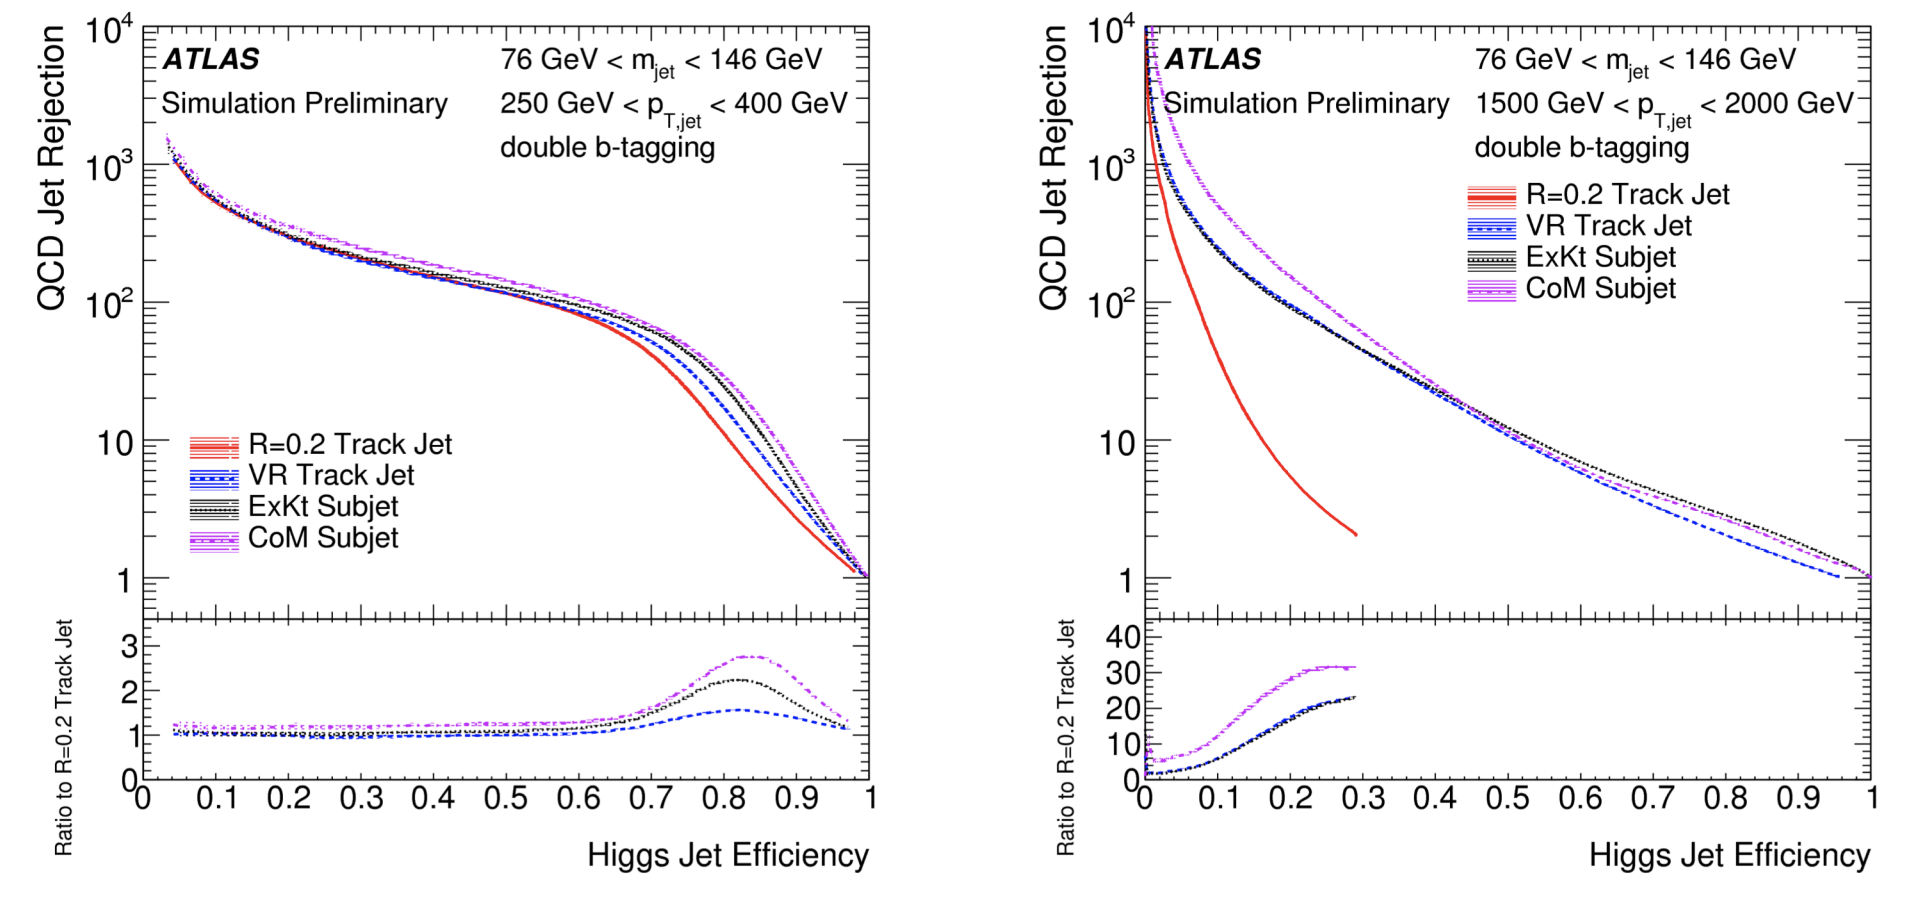
\includegraphics[width=1\textwidth]{chapters/c5/figures/higgs_ROC}
    \caption{ROC curves using four different subjet techniques: R = 0.2 track jets, VR track jets, ExKt calorimeter jets, and CoM calorimeter jets.}
    \label{fig:higgs_ROC}
\end{figure}

\par The VR track jet technique was chosen to use as subjets in the mono-Higgs analysis as an existing framework to calibrate track jets was readily available in ATLAS.












